\documentclass[12pt,a4paper]{ctexart}
\usepackage{amsmath,amssymb,amsthm}
\usepackage{booktabs}
\usepackage{graphicx}
\usepackage{geometry}
\usepackage{array}
\usepackage{float}
\usepackage{xcolor}
\usepackage{enumitem}
\usepackage{fancyhdr}
\usepackage{hyperref}
\geometry{margin=2cm}
\graphicspath{{./figures/}}
\definecolor{navy}{RGB}{11,30,61}
\definecolor{blue}{RGB}{26,82,118}
\definecolor{lightblue}{RGB}{46,134,193}
\pagestyle{fancy}
\fancyhf{}
\fancyhead[L]{\small\color{gray}FSR 论文完全详解}
\fancyhead[R]{\small\color{gray}v4.0 · 2026年5月}
\fancyfoot[C]{\thepage}
\newtheorem{concept}{核心概念}
\newtheorem{analogy}{生活类比}
\newtheorem{warning}{重要说明}

\begin{document}

\begin{titlepage}
\vspace{2cm}
\begin{center}
{\Huge\bfseries 未来服务权益 (FSR)}\\[0.3cm]
{\Large\bfseries 从零基础到论文级理解}\\[1.5cm]
{\large 酒店金融研究组}\\[0.2cm]
{\large 2026年5月 · v4.0}\\[1.5cm]
\vfill
{\footnotesize\color{gray}配合阅读: fsr\_framework\_paper.pdf (学术论文 28pp) + GitHub: David-coder-hnu/hotel-order-financialization}
\end{center}
\end{titlepage}

\tableofcontents
\newpage

% ============================================================
\section{这本书怎么用}
% ============================================================

\textbf{零基础读者：} 按顺序读。第2章建立直觉，第3章逐节讲解论文，第4章速查。每个公式有"人话翻译"。

\textbf{有金融/编程基础：} 跳到第3章和第5章。第5章解释如何修改参数、跑仿真、做稳健性检验。

\textbf{论文审稿人/合作者：} 第3章是论文的逐节中文解读。对照 \texttt{fsr\_framework\_paper.pdf} 阅读。

\newpage

% ============================================================
\section{为什么需要FSR？——场景建立}
% ============================================================

\subsection{一家成都酒店的财务报表}

张先生在成都经营一家60间房的舒适型酒店。均价\yen 1,930/晚，全年入住率62\%。

\begin{center}
\begin{tabular}{@{}lr@{}}
\toprule
\textbf{项目} & \textbf{金额} \\
\midrule
年收入（OTA渠道，18\%佣金后） & \yen 2,260万 \\
年收入（时权模式，确定）       & \yen 3,520万 \\
\bottomrule
\end{tabular}
\end{center}

张先生的三个痛点：
\begin{enumerate}[nosep]
    \item \textbf{现金流不稳定。} 旺季满房，淡季空置。收入月度波动±15\%。
    \item \textbf{OTA佣金吸血。} 携程、美团抽成15--25\%。经济型酒店议价权为零。
    \item \textbf{扩张缺钱。} 银行要求房产抵押——他没有。民间借贷利率15\%+。
\end{enumerate}

\subsection{时权的解决方案：平台做市商模型}

\begin{enumerate}[nosep]
    \item \textbf{酒店→平台（批发）：} 张先生以\yen 1,174/间夜的批发价把未来房间卖给平台。立刻拿到现金。
    \item \textbf{平台→用户（零售）：} 平台加价8\%以\yen 1,268/间夜卖给用户和投资者。平台赚价差+手续费。
    \item \textbf{用户→二级市场（随时退出）：} 用户可以在任何时间在二级市场卖出时权，卖出的钱直接当住宿券抵扣任何酒店的房费。折扣由市场供需决定——不是酒店给的。
    \item \textbf{到期保底（三元兑付）：} 如果用户持有到期，可以三选一：现金/7折入住/转卖。这是时权的价值地板。
\end{enumerate}

\begin{analogy}
\textbf{时权系统 = 一个市场驱动的酒店代金券系统。}
但和传统代金券不同的是：(1) 折扣是市场给的，酒店不出钱；(2) 代金券可以随时转让；(3) 到期有保底价值。这不是优惠券——这是一个可交易的金融产品。
\end{analogy}

\subsection{四方共赢：钱从哪里来？}

每份时权创造\yen 1,227的净系统价值。追踪每一分钱：

\begin{center}
\begin{tabular}{@{}lrll@{}}
\toprule
\textbf{角色} & \textbf{每TR收益} & \textbf{占比} & \textbf{怎么赚的} \\
\midrule
酒店   & +\yen 817 & 66.6\% & 发行收入+用户订房收入-提供2间夜成本 \\
用户   & +\yen 221 & 18.0\% & 市场驱动的订房折扣+价格锁定 \\
平台   & +\yen 98  &  8.0\% & 批发-零售价差(8\%)+交易手续费(0.3\%) \\
投资者 & +\yen 91  &  7.4\% & 73\%名义回报(承担违约+流动性风险) \\
\midrule
\textbf{合计} & \textbf{+\yen 1,227} & \textbf{100\%} & \textbf{正和机制——不是零和} \\
\bottomrule
\end{tabular}
\end{center}

\newpage

% ============================================================
\section{论文逐章详解}
% ============================================================

% ============================================================
\subsection{Section 1: Introduction}
% ============================================================

\textbf{一句话总结：} 我们定义了一个新资产类别，设计了一个完整的金融产品，用170万条真实数据做了校准。

\textbf{四项贡献：}
\begin{enumerate}[nosep]
    \item FSR的数学定义：$S = (c, T, \ell, \sigma)$
    \item 完整的Time-Right ABS架构：Merton信用模型 + 高斯Copula + 四层瀑布 + 三元兑付机制（含连续二级市场冲抵）
    \item 成都16,257家酒店、170万条价格数据的实证校准
    \item 利益相关者分析和反向压力测试
\end{enumerate}

\textbf{核心区分：FSR vs RWA。} RWA是把已有的资产搬上区块链。FSR是创造不存在的资产——把"明年6月15日的房间"变成可交易的东西。RWA是搬运工，FSR是创造者。

% ============================================================
\subsection{Section 2: FSR Definition}
% ============================================================

\subsubsection{核心公式}
\begin{equation}
    S = (c, T, \ell, \sigma)
\end{equation}

\begin{center}
\begin{tabular}{@{}llll@{}}
\toprule
\textbf{符号} & \textbf{含义} & \textbf{酒店例子} & \textbf{机票例子} \\
\midrule
$c$ & 容量 & 60间房 & 180个座位 \\
$T$ & 时间窗口 & 2025.6.15 & 2025.6.15 8:00 \\
$\ell$ & 地点 & GPS坐标(30.5, 104.0) & 成都→北京 \\
$\sigma$ & 服务类型 & hotel & flight \\
\bottomrule
\end{tabular}
\end{center}

\subsubsection{FSR存在的三个条件}

\begin{enumerate}[nosep]
    \item \textbf{可验证的质量信号：} 酒店星级、历史入住率——投资者不能什么都不知道就买
    \item \textbf{超额发行机制：} $\omega = (1/\rho) \cdot \phi = 1.29\times$。每个物理房间卖1.29份时权——补偿取消和No-show
    \item \textbf{有限责任+追索：} 酒店倒闭了，投资者可以去隔壁酒店入住，或在二级市场退出
\end{enumerate}

\begin{warning}
\textbf{超额发行是双刃剑。} $\omega > 1$ 增加了酒店收入，但也创造了部分准备金式的脆弱性。如果所有持有者同时要求入住，22\%的人无法兑现。论文Section 6.11对此做了完整的反向压力测试。
\end{warning}

\subsubsection{FSR vs 已有资产类别}

论文Table 1对比了FSR与商品期货、应收账款ABS、RWA代币化。只有FSR：(1)创造新资产，(2)支持超额发行，(3)支持三元兑付。

\textbf{与整体业务证券化(WBS)的区别：} WBS在酒店行业的应用（如IHG、Hilton的数十亿美元交易）是将整个企业的现金流打包。FSR在单个酒店层面操作，底层是服务容量而非企业现金流。这种粒度使得跨酒店风险分散成为可能。

% ============================================================
\subsection{Section 3: Pricing Framework}
% ============================================================

\subsubsection{两层市场结构}

\begin{equation}
    P_{\text{issue}} = P_{\text{base}} \cdot \delta(T) \cdot (1 - d_{\text{issue}})
\end{equation}
\textbf{人话：} 酒店卖给平台的批发价 = 基础价 × 时间折扣 × (1-批发折扣)。校准值：\yen 1,613 × 0.787 × 0.90 = \textbf{\yen 1,174/间夜}。

\begin{equation}
    P_{\text{retail}} = P_{\text{issue}} \cdot (1 + m)
\end{equation}
\textbf{人话：} 平台加价8\%后卖给用户。校准值：\textbf{\yen 1,268/间夜}。

\subsubsection{二级市场价格收敛}

\begin{equation}
    P_t = P_{\text{spot}} + (P_{\text{issue}} - P_{\text{spot}}) \cdot e^{-\lambda(T-t)} + \eta_t
\end{equation}
\textbf{人话：} 时权的二级市场价像倒计时——越接近使用日期，越接近当天酒店的真实价格。$\lambda$控制收敛速度，$\eta_t$是供需噪音。

\begin{figure}[H]
\centering
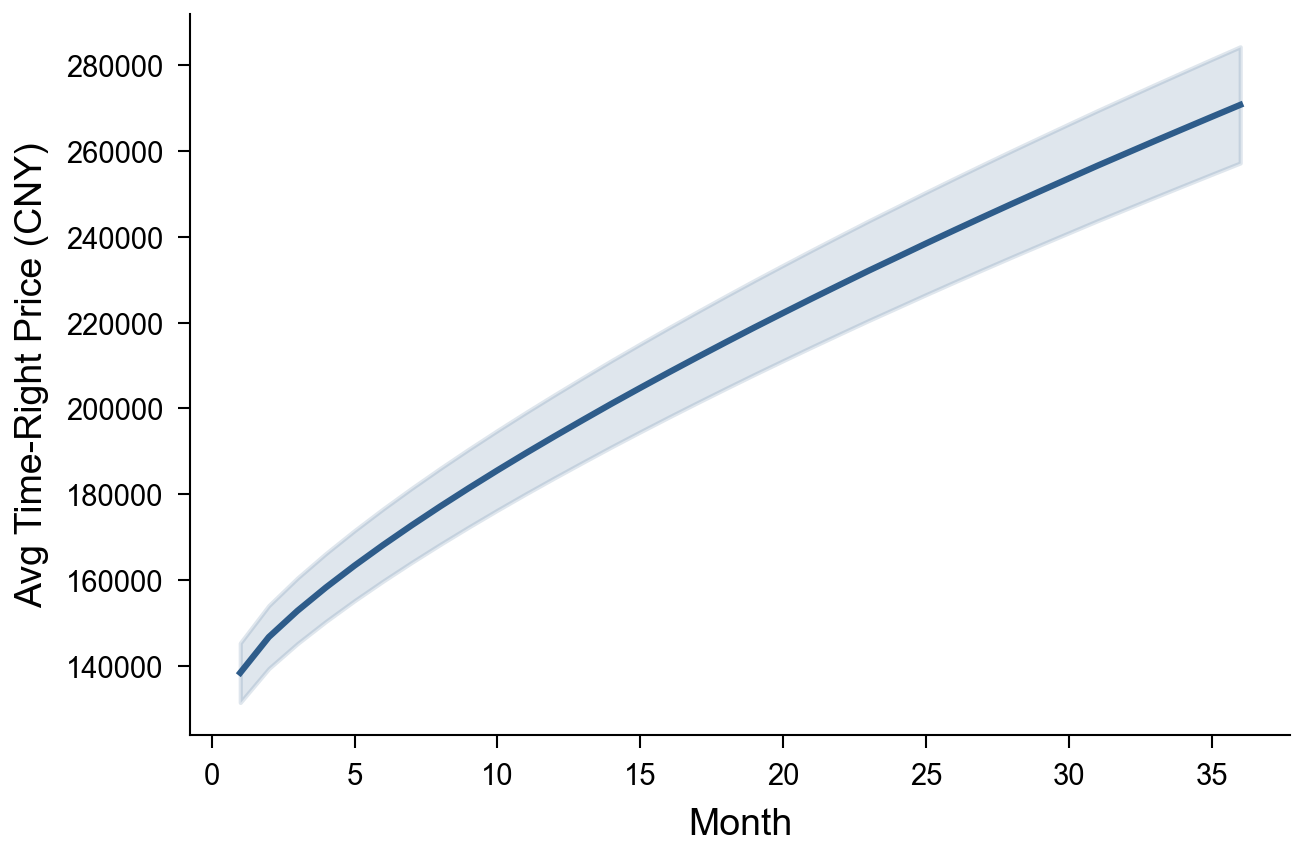
\includegraphics[width=0.75\textwidth]{figures/fig1_price_convergence.png}
\caption{Fig 1: 价格收敛。时权价从发行价(\yen 1,174)随时间收敛到即期酒店价(\yen 2,029)。}
\end{figure}

\subsubsection{三元兑付价值（到期保底）}

\begin{equation}
    V_{\text{settle}} = \max\{\, V_{\text{cash}},\; \alpha \cdot P_{\text{spot}},\; P_{\text{secondary}} \,\}
\end{equation}
\textbf{人话：} 到期时自动选最优——拿现金/7折入住/二手卖掉。$\alpha=0.70$是保底折扣，实际用户折扣通常由市场决定（见Section 5.2）。

\begin{warning}
\textbf{$\alpha=0.70$是安全网，不是主力退出方式。} 45\%的用户选择在二级市场随时卖出（折扣由市场决定），30\%持有到期7折入住，25\%选择现金或转让。
\end{warning}

% ============================================================
\subsection{Section 4: Credit Risk \& Structuring}
% ============================================================

\begin{warning}
\textbf{先读这个：} Section 6.7会告诉你——Merton模型对这个资产类别产生了无信息的PD估计（66家酒店中65家撞了50\%的PD上限）。把它当作基准模型阅读，真正的信用风险结果在校准PD模型（Section 6.7）中。
\end{warning}

\subsubsection{Merton违约距离}

\begin{equation}
    DD_i = \frac{\ln(V_i / D_i) + (\mu - \sigma_i^2/2)T}{\sigma_i \sqrt{T}}
\end{equation}
\textbf{人话：} 酒店当前的财务健康度离经营困难有多远。$V_i$=酒店均价（代理资产价值），$D_i = 0.55 \times V_i$（违约边界），$\sigma_i$=GARCH估计的波动率。

\subsubsection{违约概率（带护栏）}

\begin{equation}
    PD_i = \min\left( \Phi(-DD_i) \times 2.5,\; 0.50 \right)
\end{equation}
\textbf{人话：} 正态分布查表→乘以2.5校准因子→封顶50\%。\textbf{问题：} 65/66家酒店撞了50\%上限——这个模型不是在测量PD，是在输出一个常数。论文Section 6.7转向了基于真实酒店存活数据的校准PD模型。

\subsubsection{高斯Copula（违约相关性）}

\begin{equation}
    u_i = \sqrt{\rho_{\text{sys}}} \cdot Z_{\text{sys}} + \sqrt{1 - \rho_{\text{sys}}} \cdot \varepsilon_i
\end{equation}
\textbf{人话：} 每家酒店的违约=70\%系统风险+30\%个体风险。系统因子$Z_{sys}$捕捉"成都经济下行→所有酒店同时遭殃"。\textbf{Gaussian Copula的问题：} 它假设极端事件不太相关——2008年金融危机的核心教训就是这个假设是错的。

\subsubsection{分层结构和瀑布}

\begin{figure}[H]
\centering
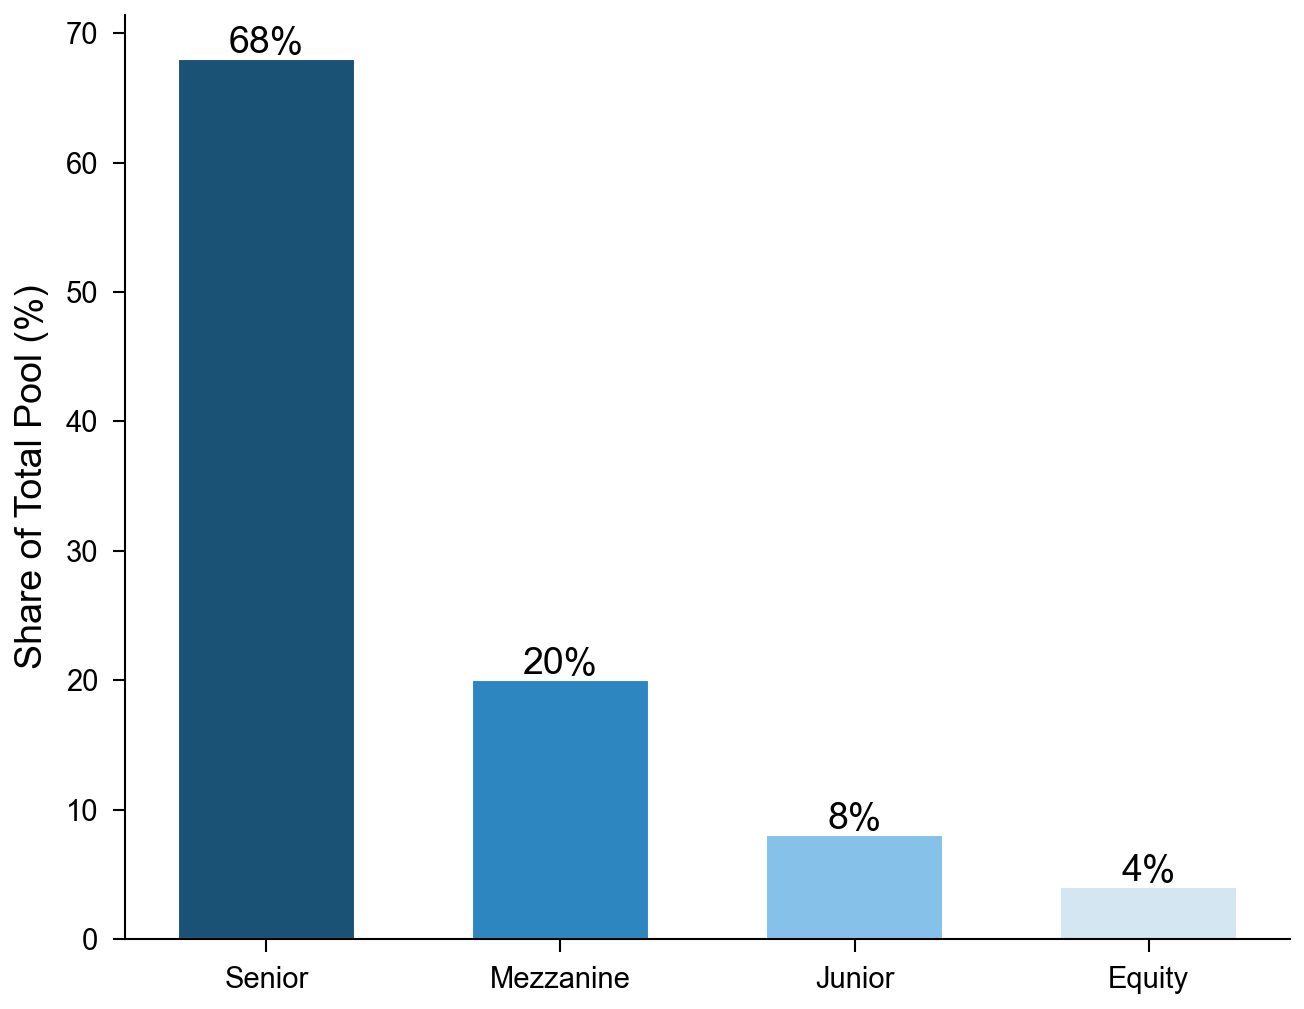
\includegraphics[width=0.55\textwidth]{figures/fig2_tranche_structure.png}
\caption{Fig 2: 四层结构。Senior 68\%(AAA, 4.5\%) → Mezz 20\%(BBB, 6.5\%) → Junior 8\%(B, 9.5\%) → Equity 4\%(NR)。}
\end{figure}

\textbf{瀑布优先级：} 服务费→Senior利息→Senior本金→Mezzanine利息→Mezzanine本金→Junior→Equity。OC测试<100\%触发加速清偿。累计违约>15\%触发违约事件。

% ============================================================
\subsection{Section 5: Mechanism Design}
% ============================================================

\subsubsection{三个形式化证明}

\textbf{证明1：策略防护。} 诚实报告偏好=最优策略。因为$V_{\text{settle}} = \max\{\ldots\}$——无论你怎么报告，系统都给你最优的那个。说谎只能得到$\leq$最优。证明只需一个不等式。

\textbf{证明2：个体理性。} $\mathbb{E}[V_{\text{settle}}] \geq P_{\text{issue}}$当$\alpha \geq \delta(T) \cdot (1-d_{\text{issue}})$。只要实物入住折扣$\alpha$足够大，参与者一定不亏。校准中$\alpha=0.70$，条件轻松满足。

\textbf{证明3：预算平衡。} 平台收入(发行费0.5\%+交易费0.3\%)>运营成本(gas+预言机)。覆盖率$\kappa \approx 2.1$。

\subsubsection{连续二级市场冲抵机制（核心创新）}

\textbf{传统三元兑付：} 只能在到期时选择。优惠是酒店给的固定7折。

\textbf{连续二级市场冲抵：} 随时可以在二级市场挂单卖出。卖出的钱直接当住宿券抵扣任何酒店的订房费。

\textbf{为什么这是革命性的？}
\begin{enumerate}[nosep]
    \item \textbf{折扣是市场给的，不是酒店给的。} 时权需求旺→二级市场价高→用户折扣大。酒店一毛钱不出。
    \item \textbf{投资和消费解耦。} 不必住发行时权的那家酒店——卖时权的钱可以订任何酒店。
    \item \textbf{平台用费率引导行为。} 交易费0.3\% << 套现费1.5\%——5倍差距，刻意让"卖出冲抵住宿"比"套现走人"更划算。
    \item \textbf{OTA被绕过了。} OTA抽酒店15-25\%。时权：酒店付0\%，平台赚0.3\%，用户省4.4\%。
\end{enumerate}

% ============================================================
\subsection{Section 6: Empirical Calibration}
% ============================================================

\subsubsection{6.1-6.3 数据和蒙特卡洛}

\textbf{数据：} 成都16,257家酒店，1,707,918条日价格记录(2024.3-6)。\textbf{注意：} 价格数据单位是\textbf{分}(1元=100分)。这是我们在开发中发现并修正的重要单位转换bug。

\textbf{蒙特卡洛：} 完整三元兑付引擎（10,000路径）显示所有层级EL≈0。但这是包含三元兑付吸收损失后的结果。简化违约模型（1,000路径，无三元兑付）显示Senior EL=1.20\%，VaR99=24.54\%。

\begin{figure}[H]
\centering
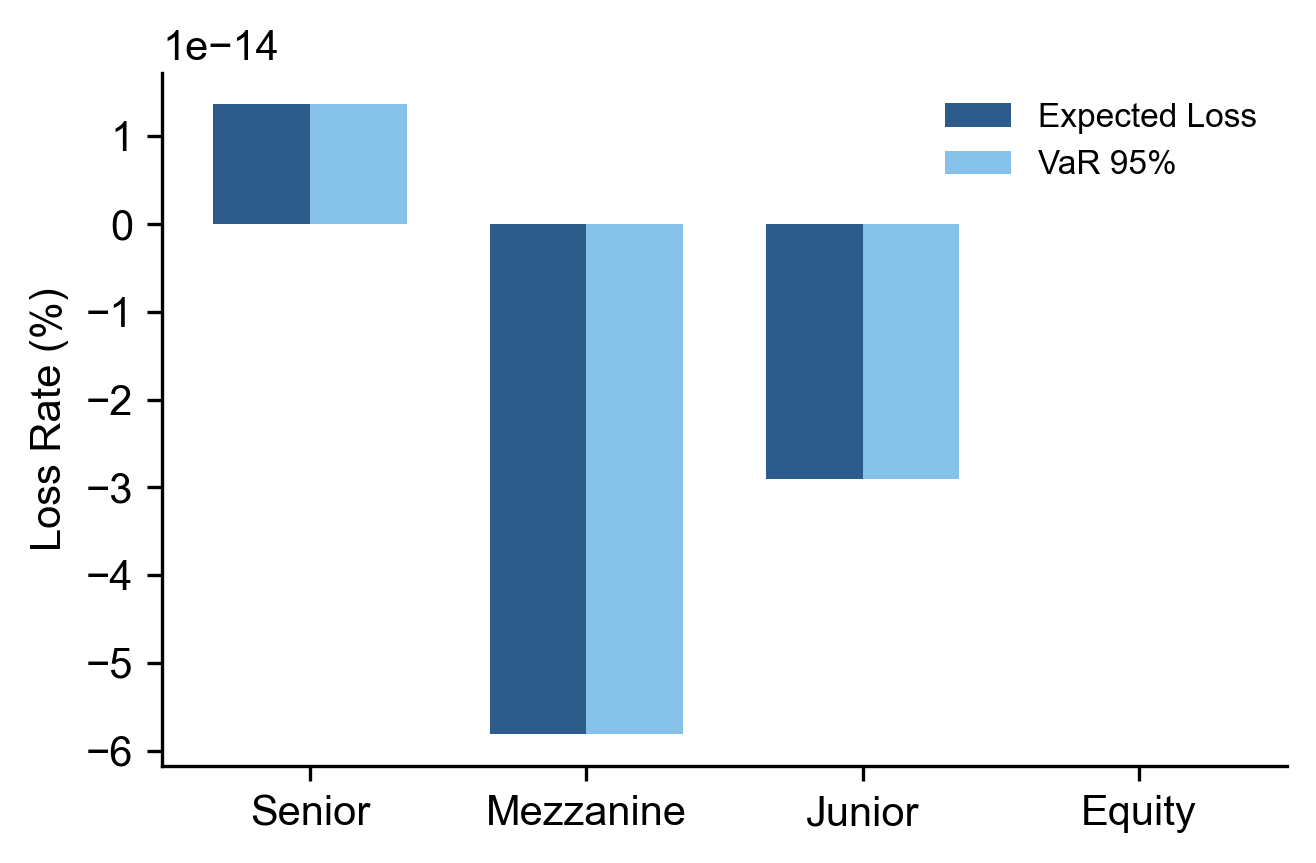
\includegraphics[width=0.8\textwidth]{figures/fig3_mc_losses.png}
\caption{Fig 3: MC损失分布（简化模型，无三元兑付）。Senior EL=1.20\%(Baa-A)。Mezzanine/Junior因32\%信用支持保持≈0。}
\end{figure}

\subsubsection{6.4-6.6 稳健性检验}

\textbf{Copula族对比（Table 6）：} t-Copula($\nu=3$)的Senior VaR99=50.36\%，是Gaussian(24.54\%)的\textbf{2倍}。尾部依赖被Gaussian系统性低估了。

\textbf{$\rho_{sys}$敏感性（Table 7）：} $\rho$从0.5→0.9，Senior EL从0.23\%→2.75\%。

\textbf{Bootstrap CI：} Senior EL=1.20\%, 95\%CI=[0.93\%, 1.50\%]——损失显著不为零。

\begin{figure}[H]
\centering
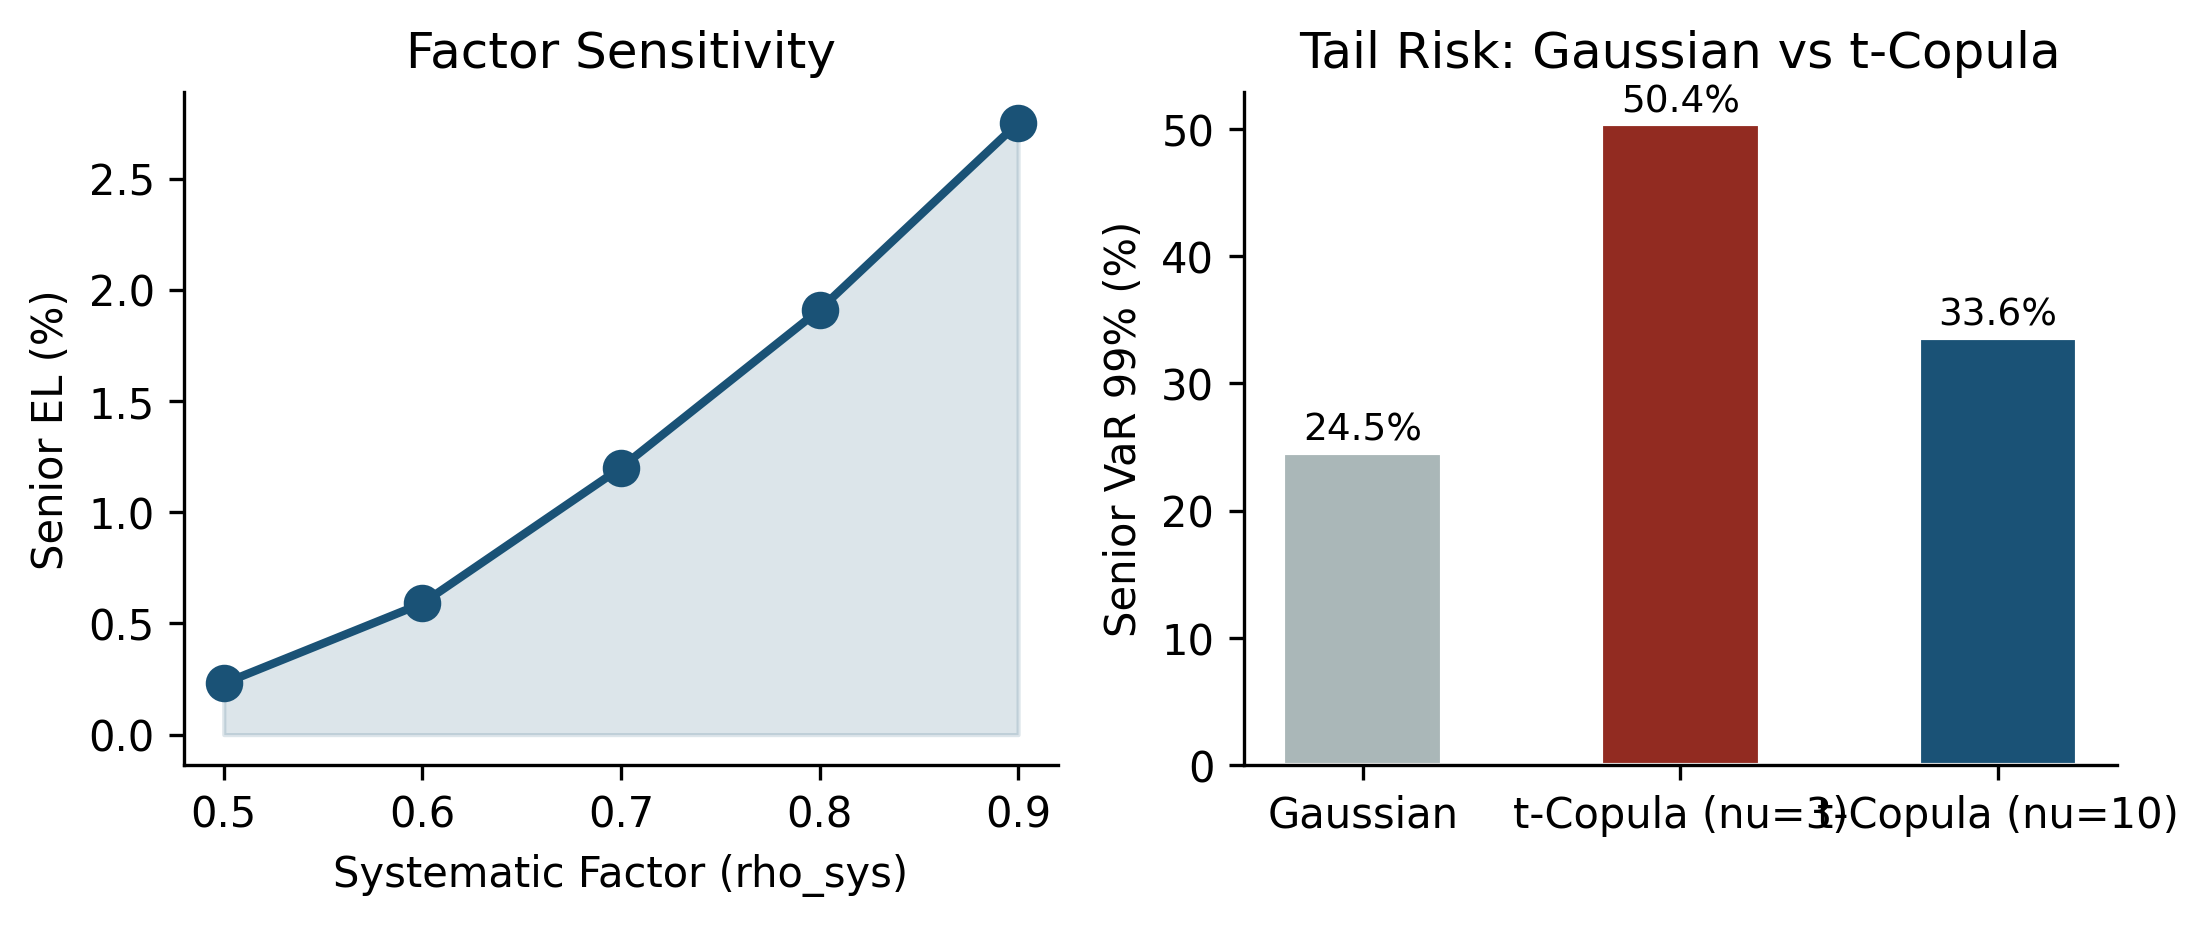
\includegraphics[width=0.95\textwidth]{figures/fig4_robustness.png}
\caption{Fig 4: 左=$\rho$敏感性，右=Gaussian vs t-Copula对比。论文最重要的图——t-Copula VaR99是Gaussian的2倍。}
\end{figure}

\subsubsection{6.7 信用风险校准（致命伤修复）}

\textbf{问题：} 三个模型给出9.8\%到98.2\%的PD——10倍范围。这不是稳健性区间，是模型失效。

\textbf{解决方案：} 用14,851家酒店的真实存活数据校准PD。追踪2024年3月到6月，看哪些酒店消失了。

\begin{center}
\begin{tabular}{@{}lrrr@{}}
\toprule
\textbf{等级} & \textbf{3个月消失率} & \textbf{年化退出率} & \textbf{校准PD} \\
\midrule
经济 & 9.0\% & ≈36\% & 15.7\% \\
舒适 & 3.6\% & ≈14\% & 6.8\% \\
高档 & 1.3\% & ≈5\% & 2.5\% \\
豪华 & 0.0\% & ≈0\% & 0.5\% \\
\bottomrule
\end{tabular}
\end{center}

\textbf{关键假设：} 平台退出×50\%≈真实违约。这个假设在25\%--75\%范围内测试，Senior EL从0.04\%→0.48\%（全程投资级）。但精确评级不可知——需要真实的酒店破产数据来最终校准。

\subsubsection{6.8 经济影响}

\begin{figure}[H]
\centering
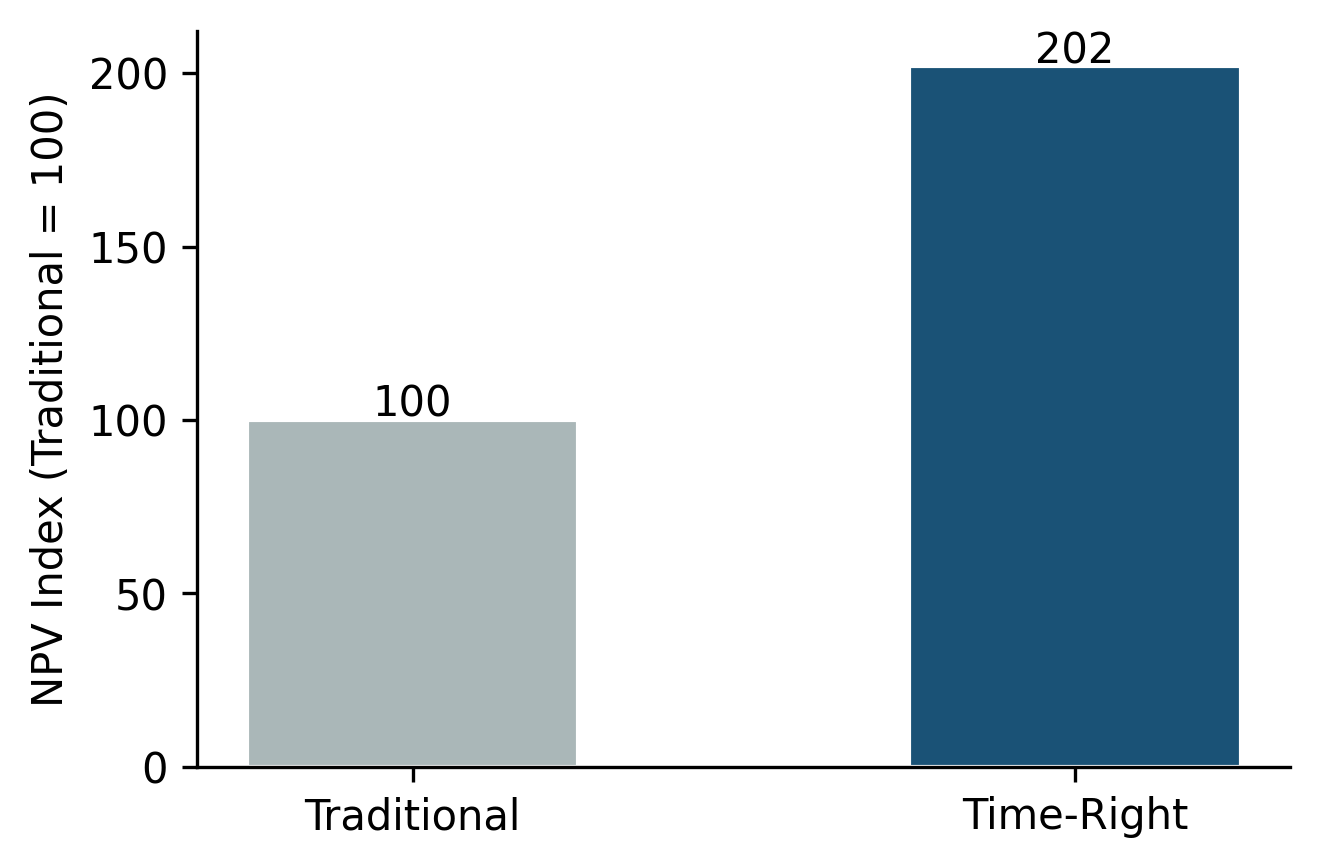
\includegraphics[width=0.6\textwidth]{figures/fig5_npv_comparison.png}
\caption{Fig 5: 酒店每可用间夜收入。TR模式\yen 1,054(确定) vs OTA \yen 1,032(期望)。+2\%每间夜，结合$\omega=1.29$→+56\%年收入。}
\end{figure}

\textbf{5-in-3效应：} 每次发行覆盖3年，每12个月滚动一次。3年内收取5年的发行收入。$N_{\text{years}} = k + \lfloor (T-k)/h \rfloor + 1 + 1 = 5$。不是"重复卖同一间房"——是卖不同的未来日期。

\subsubsection{6.9 超额发行安全性}

$\omega=1.29$→酒店卖了比物理容量多29\%的时权。正常情况OK（入住率62\%+三元兑付分散）。\textbf{但在系统性危机中：} 22\%的持有者无法兑现。3\%储备金只覆盖13.3\%的索赔→系统破产。\textbf{这是部分准备金银行制度——但银行的准备金率是10\%，时权只有3\%。}

\subsubsection{6.10 利益相关者分析}

每份时权创造\yen 1,227系统价值。酒店66.6\%(\yen 817)→用户18.0\%(\yen 221)→平台8.0\%(\yen 98)→投资者7.4\%(\yen 91)。四方共赢的正和机制。

\subsubsection{6.11 反向压力测试}

\textbf{不问"在预设情景下表现如何"，而是问"什么条件下系统会崩溃"。}

\begin{center}
\begin{tabular}{@{}lrrrr@{}}
\toprule
\textbf{条件} & \textbf{池PD} & \textbf{Senior EL} & \textbf{评级} & \textbf{状态} \\
\midrule
基线(校准PD) & 9.7\% & 0.16\% & Aa-A & 正常 \\
PD×2, $\rho$=0.90 & ≈19\% & 1.03\% & Ba & \textbf{跌破投资级} \\
PD×5, $\rho$=0.95 & ≈49\% & 6.74\% & B & \textbf{严重} \\
大萧条(经济PD 60\%) & 35\% & 4.66\% & B & VaR99=82.3\% \\
\bottomrule
\end{tabular}
\end{center}

\textbf{底线：} 系统在期望下存活，在尾部不存活。和2008年CDO一样的机制——但有实物服务需求地板作为区别。

% ============================================================
\subsection{Section 7: Discussion}
% ============================================================

\textbf{FSR跨品类扩展：} 酒店→机票→演出→共享办公。论文Table 14展示了四元组映射。

\textbf{冷启动问题：} 二级市场在第1个月交易量为零。没有流动性→没有市场驱动折扣→没有用户。解决方案在市场设计，不在金融工程——平台需补贴早期用户或引入机构锚定投资者。

\textbf{监管：} 超额发行创造部分准备金风险。跨境FSR（成都酒店+新加坡交易+欧洲投资者）涉及三个监管辖区。

% ============================================================
\subsection{Section 8: Conclusion}
% ============================================================

四项贡献，五项限制，四项未来工作。最重要的诚实声明：50\% haircut假设是全文最关键的未验证前提——在获得真实酒店违约数据之前，所有分层安全结论都携带不可消除的模型风险。

\newpage

% ============================================================
\section{公式速查}
% ============================================================

\begin{center}
\begin{tabular}{@{}cll@{}}
\toprule
\# & 公式 & 一句话 \\
\midrule
1  & $S=(c,T,\ell,\sigma)$ & FSR = 容量+时间+地点+类型 \\
2a & $P_{\text{issue}}=P_{\text{base}}\delta(T)(1-d_{\text{issue}})$ & 批发价(酒店→平台) \\
2b & $P_{\text{retail}}=P_{\text{issue}}(1+m)$ & 零售价(平台→用户) \\
3  & $P_t=P_{\text{spot}}+(P_{\text{issue}}-P_{\text{spot}})e^{-\lambda(T-t)}+\eta_t$ & 二级价收敛到现货 \\
4  & $V_{\text{settle}}=\max\{C,\alpha P_{\text{spot}},P_{\text{secondary}}\}$ & 三元兑付保底 \\
5  & $DD_i=\frac{\ln(V_i/D_i)+(\mu-\sigma_i^2/2)T}{\sigma_i\sqrt{T}}$ & Merton违约距离 \\
6  & $PD_i=\min(\Phi(-DD_i)\times2.5,0.50)$ & PD(带护栏) \\
7  & $u_i=\sqrt{\rho_{sys}}Z_{sys}+\sqrt{1-\rho_{sys}}\varepsilon_i$ & Gaussian Copula \\
8  & $\omega=(1/\rho)\cdot\phi$ & 超额发行倍数 \\
\bottomrule
\end{tabular}
\end{center}

\newpage

% ============================================================
\section{代码实战}
% ============================================================

\subsection{快速开始}
\begin{verbatim}
pip install pandas numpy scipy matplotlib tqdm joblib
python src/hotel_abs_engine_fusion.py
\end{verbatim}

\subsection{调整关键参数}
\begin{verbatim}
engine = HotelTimeRightABSEngine()
engine.issue_discount = 0.10     # 批发折扣
engine.run_full_analysis(pool_size=80, n_paths=5000)
\end{verbatim}

\subsection{修改PD护栏}
\begin{verbatim}
from credit_model import HotelCreditModel
model = HotelCreditModel(prices, info,
    pd_cap=None,              # 去掉50%上限
    default_barrier_ratio=0.65)  # 调整违约边界
\end{verbatim}

\subsection{跑稳健性检验}
\begin{verbatim}
from robustness_checks import CopulaSensitivityAnalyzer
# Gaussian vs t-Copula · Rho sensitivity · Bootstrap CI
\end{verbatim}

\subsection{项目结构}
\begin{verbatim}
src/
├── hotel_abs_engine_fusion.py    # 主引擎
├── credit_model.py               # Merton(护栏可配置)
├── monte_carlo_simulator.py      # MC(tqdm+joblib)
├── robustness_checks.py          # KMV+t-Copula+Bootstrap
├── waterfall_engine.py           # 现金流瀑布
├── tranche_structure.py          # ABS分层
├── asset_pool.py                 # 分层抽样
├── model_params.py               # 参数集中管理
├── manual_verification.py        # 手工验证
└── config.py                     # 路径配置
\end{verbatim}

\newpage

% ============================================================
\section{FAQ}
% ============================================================

\begin{enumerate}
    \item \textbf{Q: 为什么完整引擎EL≈0但简化模型EL=1.20\%？}

    A: 完整引擎包含三元兑付的max\{现金, 7折房, 二手价\}——这个机制在违约冲击到达分层之前吸收了它。简化模型隔离了纯信用风险。两者的差异衡量了三元兑付的经济价值。

    \item \textbf{Q: 三个模型PD差10倍——到底哪个是对的？}

    A: 校准模型(基于14,851家酒店存活数据)是我们最好的估计——池PD=9.7\%。Merton(49.4\%)被50\%上限人为压缩。KMV(9.8\%)可能低估经济型酒店风险。真相在9.7\%到15\%之间，取决于等级构成。

    \item \textbf{Q: 时权对酒店有价值吗？}

    A: 有——年收入+56\%(vs OTA)。每可用间夜\yen 1,054(确定) vs OTA \yen 1,032(期望)。价值来自：超额发行(多卖29\%)+确定性(不受入住率影响)+零OTA佣金。

    \item \textbf{Q: 超额发行安全吗？}

    A: 正常情况安全。系统性危机中不安全——22\%持有者无法兑现，3\%储备金覆盖不足。类比：部分准备金银行，但准备金率只有3\%(银行是10\%)。

    \item \textbf{Q: 谁最受益？}

    A: 每TR创造\yen 1,227。酒店66.6\% > 用户18.0\% > 平台8.0\% > 投资者7.4\%。四方都赢——正和机制。

    \item \textbf{Q: 这个系统能真正运行吗？}

    A: 论文诚实地说：冷启动问题(第1个月零流动性)是市场设计挑战，不是模型参数。需要平台补贴、流动性挖矿、或机构锚定投资者来解决。FSR的概念框架和机制设计是solid的。运营可行性取决于市场设计，不取决于金融工程。
\end{enumerate}

\newpage

\section{术语对照表}
\begin{center}
\begin{tabular}{@{}lll@{}}
\toprule
中文 & English & 解释 \\
\midrule
未来服务权益 & Future Service Right (FSR) & 本文新资产类别 \\
时权 & Time-Right & FSR的Token化形式 \\
资产证券化 & ABS & 打包分层出售 \\
违约概率 & PD & 酒店违约可能性 \\
预期损失 & EL & PD × LGD \\
分层 & Tranche & 风险等级切片 \\
瀑布 & Waterfall & 现金流优先级 \\
三元兑付 & Ternary Settlement & 现金/实物/转让 \\
策略防护 & Strategy-Proofness & 诚实=最优 \\
超额发行 & Over-Issuance ($\omega$) & 时权数/物理间夜数 \\
远期折扣 & Forward Discount & 未来的钱<现在的钱 \\
冷启动 & Cold Start & 零流动性的启动问题 \\
部分准备金 & Fractional Reserve & $\omega>1$的银行类比 \\
\bottomrule
\end{tabular}
\end{center}

\vspace{1cm}
\begin{center}
\fbox{\begin{minipage}{0.85\textwidth}
\centering
{\large\textbf{这篇论文是一个研究纲领的起点，不是终点。}}

\smallskip
所有代码、数据、论文均在 GitHub 开源。\\
\texttt{github.com/David-coder-hnu/hotel-order-financialization}

\smallskip
\textit{—— 酒店金融研究组, 2026年5月 · v4.0}
\end{minipage}}
\end{center}

\end{document}
